\documentclass[10pt, conference, compsocconf]{IEEEtran}

% packages
\usepackage{algorithm}
\usepackage{algorithmic}
\usepackage{amsfonts} % for R symbol (the set of real numbers)
\usepackage{color}
\usepackage[pdftex]{graphicx}
\usepackage{graphicx}
\usepackage[bookmarks=false]{hyperref}
\hypersetup{colorlinks=true,linkcolor=black,citecolor=black,filecolor=black,urlcolor=blue}
\usepackage{mathtools}
\usepackage{multirow}
\usepackage{stmaryrd} % for llbracket and rrbracket
\usepackage{subcaption}
\usepackage{nicefrac}
\usepackage{amsmath}
\DeclarePairedDelimiter{\ceil}{\lceil}{\rceil}
\DeclarePairedDelimiter{\floor}{\lfloor}{\rfloor}

% new commands
\newcommand{\todo}[1]{\marginpar{\parbox{18mm}{\flushleft\tiny\color{red}\textbf{TODO}:
      #1}}}
\newcommand{\comment}[1]{\marginpar{\parbox{18mm}{\flushleft\tiny\color{blue}\textbf{Comment}:
      #1}}}

\newcommand{\note}[1]{
  \color{blue}\emph{[Note: #1]}
  \color{black}
}

\begin{document}

\title{Predicting computational reproducibility of data analysis pipelines \\in large population studies using collaborative filtering}

\author{Soudabeh Barghi, Lalet Scaria, Tristan Glatard\\
  Department of Computer Science and Software Engineering\\ Concordia University, Montreal, Quebec, Canada\\
  {first.last}@concordia.ca}

\maketitle

\begin{abstract}
With the rise of the reproducibility crisis, evaluating the 
computational reproducibility of data analysis pipelines has become a 
critical issue. It is, however, a cumbersome 
process for analyses that involve data from large populations of 
subjects, due to their computational and storage requirements. 
We present a method to predict the computational 
reproducibility of data analysis pipelines in large population studies. 
We formulate the problem as a collaborative filtering process, with 
constraints on the construction of the training set. We propose 6 
different strategies to build the training set, which we evaluate on 2 
datasets, a synthetic one modeling a population with a growing number 
of subject types, and a real one obtained with neuroinformatics 
pipelines. Results show that one sampling method, ``Random File Numbers 
(Uniform)" is able to predict computational reproducibility with a good 
accuracy. We also analyze the relevance of including file and subject 
biases in the collaborative filtering model. We conclude that the 
proposed method is able to speed-up reproducibility 
evaluations substantially, with a reduced accuracy loss.
\end{abstract}

\section{Introduction}

Computational reproducibility, the ability to recompute data analyses 
over time and 
space~\cite{peng2011reproducible}, has become a critical component of 
scientific methodology as many researchers acknowledge the existence of 
a reproducibility crisis~\cite{baker2016there}. Among other factors, 
such as data and code sharing, infrastructural characteristics 
play an important role in making experiments reproducible. For instance, in 
neuroinformatics, our primary field of interest, several studies have 
shown the effect of the 
operating system on computational 
results~\cite{gronenschild2012effects, glatard2015reproducibility}.
However, conducting such reproducibility studies at scale is cumbersome 
due to the computational and storage requirements of data analysis 
pipelines.

Neuroinformatics pipelines are generally iterated on data coming from 10 to 
1,000 subjects, possibly with subtle input parameter variations to 
adjust specific data acquisition conditions. Subject data often capture 
anatomical and functional characteristics of their brain, for instance through
Magnetic Resonance Imaging (MRI) or Electroencephalography (EEG). The number of files 
associated with a subject may vary, and these files may also be of 
different sizes. Typical data processing times range from 15 minutes to 
15 hours per subject, with input ranging from 100~MB to 15~GB per subject, and 
outputs ranging from 1~GB to 500~GB.

The reproducibility of a given pipeline may vary across subjects, for 
instance due to different pipeline branches being executed depending on 
the nature, cardinality or content of the input data. For instance, in 
the public database released by the Human Connectome 
Project~\cite{van2013wu}, subjects may have one or two anatomical images of 
each modality; when two images are 
present, they are aligned together and averaged. The presence of 
artifacts, for instance due to high motion during the acquisition, may 
also trigger corrections that are not otherwise required. Some branches 
of the pipeline may also be executed only for specific acquisition 
parameters, for instance the intensity of the magnetic field. To 
capture all these variations, reproducibility evaluations need to be 
conducted on many subjects, which is unwieldy. 

Our goal is to predict the outcome of reproducibility evaluations in a 
large population of subjects, from a reduced set of pipeline 
executions. More precisely, we aim at predicting whether a particular 
file produced by an analysis pipeline will be identical across 
execution conditions, or if it will contain reproducibility 
\emph{errors}. We approach the problem from the point of view of 
collaborative filtering, inspired by previous examples that applied 
this method outside of its initial application domain, for instance 
~\cite{feng2013efficient}. The main issue, and originality, of our 
problem lies in the fact that the training set cannot be arbitrarily 
sampled from the utility matrix. Instead, the training set has to 
respect the time constraints imposed by the order in which files 
are produced during pipeline executions.

This paper makes the following contributions:
\begin{enumerate}
\item We model reproducibility evaluations in data processing pipelines as a collaborative filtering problem.
\item We propose strategies to sample the training set under time constraints.
\item We evaluate and compare our sampling strategies on synthetic and real datasets.
\end{enumerate}
The problem formulation, collaborative filtering technique used, and 
proposed sampling strategies for the training set are presented in 
Section~\ref{sec:methods}. The datasets are described in 
Section~\ref{sec:datasets}, and experimental results are reported in 
Section~\ref{sec:results}.
The paper ends with a discussion about the impact, limitations and 
generalizability of our results.

\section{Method}
\label{sec:methods}
\subsection{Problem formulation}

The pipeline to be evaluated is represented by a matrix $U$ of size 
$N_f \times N_s$, where the $N_s$ columns represent data coming from 
different subjects, and the $N_f$ rows represent the files produced by 
the pipeline execution. While subjects are not ordered, files are, for 
instance from their last modification time in a sequential execution, 
and we assume that this order is consistent across subjects. $U_{i, j}$ 
measures the reproducibility of file $i$ produced during the processing 
of subject $j$ in two conditions, for instance two different 
operating systems. In our experiments, we restrict $U_{i,j}$ to be 
boolean, but our methods can be applied for real values as well. 

Our goal is to predict the test set $\mathbb{T'}$ of missing values of 
$U$ from a training set $\mathbb{T}$ of known ones, where $\mathbb{T} 
\cap \mathbb{T'} = \emptyset$ and $\mathbb{T} \cup \mathbb{T'} = 
\{U_{i,j}\}$. In contrast with the traditional collaborative filtering 
problem, (1) we have control over the construction of the training set, 
for instance we can choose to include only files producde by specific 
subjects, or the first files produced by the processing of every 
subject, and (2) the construction of the training set is constrained by 
the 
order on the matrix rows, which is formalized as follows: 
\begin{equation}
\begin{array}{l}
\forall (i, j, k) \in \llbracket 1, N_f \rrbracket \times \llbracket 1, N_f \rrbracket \times \llbracket 1, N_s \rrbracket, \\
 \left( U_{i,k} \in \mathbb{T} \quad \mathrm{and} \quad U_{j,k} \in \mathbb{T'} \right) \Rightarrow i < j. \label{eq:time}
 \end{array}
\end{equation}

Our problem is the following:
\begin{quote}
Given a training ratio $\alpha$, find a subset $\mathbb{T}$ of 
$\{U_{i,j}\}$ of size $\alpha N_f N_s$ such that (1) $\mathbb{T}$ and 
$\mathbb{T'}$ respect Equation~\ref{eq:time}, and (2) $\mathbb{T'}$ can 
be predicted from $\mathbb{T}$ with high accuracy.
\end{quote}
The sampling of the training set will be described in Section~\ref{sec:training}.
The collaborative filtering techniques used for the predictions are reported hereafter.

\subsection{Collaborative filtering}

Collaborative filtering is a technique to predict unknown values of a 
matrix called ``utility matrix" from the known ones. Traditionally, the 
matrix represents the ratings of items, represented in columns, by 
users, represented in rows. Ratings might be explicit, when users 
provide ratings through a dedicated system, or implicit, when users' 
behaviors are tracked and analyzed to estimate their preferences. An 
overview of collaborative filtering is provided 
in~\cite{leskovec2014mining}. In our context, the utility matrix is the
pipeline matrix $U$ described previously.

Several methods have been proposed to implement collaborative 
filtering. Item-item collaborative filtering~\cite{breese1998empirical, linden2003amazon} predicts 
the rating of item $i$ by user $u$ from the ratings of items similar to 
$i$ by user $u$. Likewise, user-user collaborative 
filtering~\cite{breese1998empirical} predicts the rating of item $i$ by user $u$ 
from the ratings of item $i$ by users similar to $u$. Both methods
have been used extensively for e-commerce applications.

A third class of methods, which is the one that we will apply to our 
problem, is based on the factorization of the utility matrix to 
estimate latent factors along which users and items are represented. 
This method is described 
in~\cite{koren2009matrix} and became famous as it contributed to winning the 
Netflix prize in 2009. To summarize, the method aims at finding $q_i$ 
and $p_u$ vectors of $\mathbb{R}^f$, where $f$ is the number of latent factors, such that:
\begin{equation*}
r_{ui} = q_i^Tp_u,
\end{equation*}
where $r_{ui}$ is the rating of item $i$ by user $u$. In practice, the optimization
involves a regularization term to avoid overfiting particular users or items. The method
finds $q_i$ and $p_u$ that minimize the following objective:
\begin{equation*}
\sum_{(i,u) \in \mathbb{T}}\left( r_{ui} - q_i^Tp_u\right)^2+\lambda \left( \|{q_i}\|^2 + \|{p_u}\|^2\right)
,
\end{equation*}
where $\lambda$ is the regularization parameter and $\mathbb{T}$ is the training set.

It is also common to include user biases $b_u$ and item biases $b_i$ in 
the optimization, defined as the average deviation of user $u$ and item 
$i$ to the global average $\mu$. The goal then becomes to find $q_i$ and $p_u$ that minimize the 
following objective:
\begin{equation*}
\sum_{(i,u) \in \mathbb{T}}\left( r_{ui} - \mu - b_u - b_i - q_i^Tp_u\right)^2+\lambda \left( \|{q_i}\|^2 + \|{p_u}\|^2 + b_u^2 + b_i^2\right)
\end{equation*}

Two good techniques to perform the optimization are stochastic gradient 
descent and alternating least squares (ALS). In the remainder of this 
paper, we use matrix factorization as implemented in Apache Spark's 
MLLib version 2.3.0, which uses ALS. We round predictions to the 
nearest integer to obtain binary values.


\subsection{Sampling of the training set}

\label{sec:training}

As explained before, the training set in our problem cannot be 
constructed by unconstrained random sampling of the matrix. Instead, 
the training and test sets have to comply to Equation~\ref{eq:time}. To 
address this issue, we investigated the following sampling techniques, illustrated in
Figure~\ref{fig:sampling}. 

\paragraph{Complete Columns 
(Figure~\ref{fig:Columns-Sample-Training-set})} The training set is 
sampled by randomly selecting complete columns in the utility matrix, 
that is, complete subject executions. The last selected column might be 
incomplete to meet the exact training ratio. This method respects the 
time constraints. It corresponds to a situation where the collaborative 
filtering method will predict the reproducibility of the subjects in 
the test set from the subjects in the training set. 

\paragraph{Complete Rows (Figure~\ref{fig:Rows-Sample-Training-set})} 
The training set is sampled by selecting complete rows in the utility 
matrix, that is, the first files produced by every execution. The last 
selected row might be incomplete to meet the exact training ratio. This 
method respects the time constraints. It corresponds to a situation 
where the processing of all the subjects is launched and interrupted 
before the execution is complete. The collaborative filtering method 
will then predict the reproducibility of the remaining files.

\begin{figure}[h!]
        \centering
        \begin{subfigure}[b]{0.45\columnwidth}
                  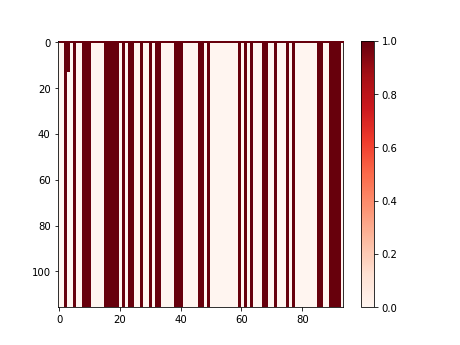
\includegraphics[width=\columnwidth]{figures/5vs7_columns_04_training}
                  \caption{Complete Columns}
                  \label{fig:Columns-Sample-Training-set}
        \end{subfigure}
        \begin{subfigure}[b]{0.45\columnwidth}
                  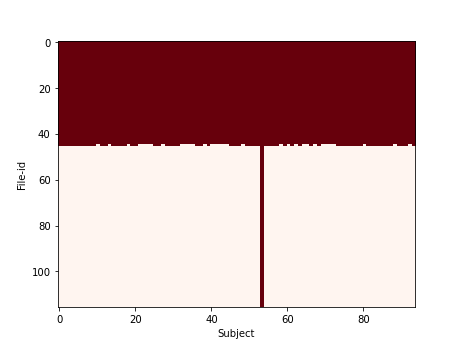
\includegraphics[width=\columnwidth]{figures/5vs7_rows_04_training}
                  \caption{Complete Rows}
                  \label{fig:Rows-Sample-Training-set}
        \end{subfigure}
        \begin{subfigure}[b]{0.45\columnwidth}
                 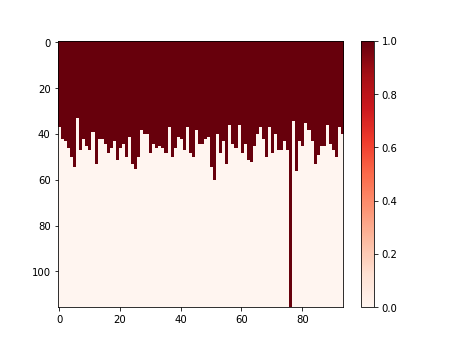
\includegraphics[width=\columnwidth]{figures/5vs7_random-real_04_training}
                \caption{Random Subjects (RS)}
                  \label{fig:Uniform-S-Sample-Training-set}
        \end{subfigure}
        \begin{subfigure}[b]{0.45\columnwidth}
                  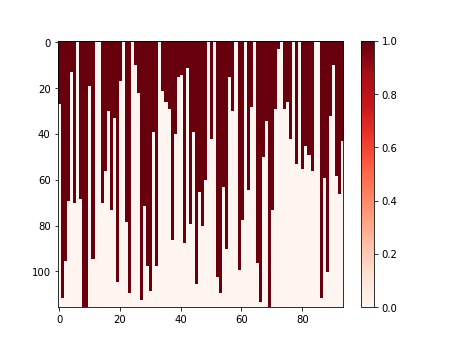
\includegraphics[width=\columnwidth]{figures/5vs7_diagonal_04_training}
                  \caption{RFNU}
                  \label{fig:Diagonal-Sample-Training-set}
        \end{subfigure}
        \begin{subfigure}[b]{0.45\columnwidth}
                  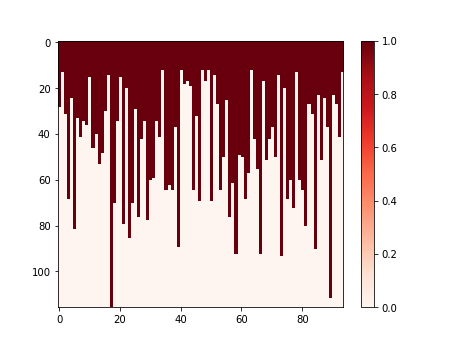
\includegraphics[width=\columnwidth]{figures/5vs7_random-triangular-largest_04_training}
                  \caption{RFNTL}
                  \label{fig:triangular-L-Sample-Training-set}
        \end{subfigure}
        \begin{subfigure}[b]{0.45\columnwidth}
                  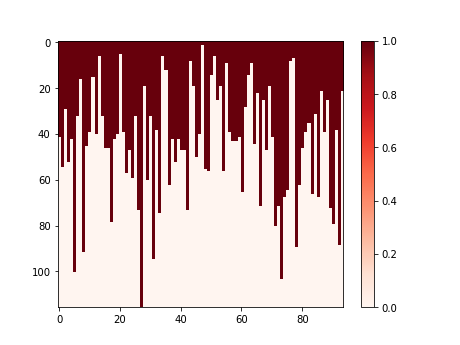
\includegraphics[width=\columnwidth]{figures/5vs7_random-triangular-smallest_04_training}
                  \caption{RFNTS}
                  \label{fig:triangular-S-Sample-Training-set}
        \end{subfigure}
        \begin{subfigure}[b]{\columnwidth}
        \centering
        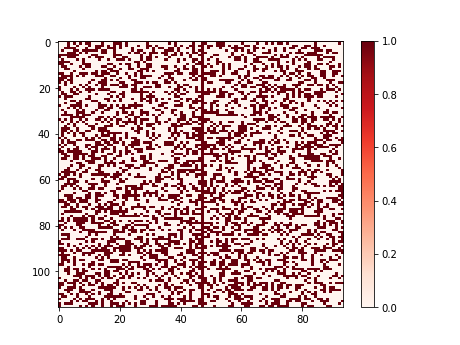
\includegraphics[width=0.45\columnwidth]{figures/5vs7_random-unreal_04_training}
                  \caption{Random Unreal}
                  \label{fig:Random-Unreal-Sample-Training-set}
        \end{subfigure}
        \caption{Sample training set for different methods with a training ratio of 0.4.}
        \label{fig:sampling}
\end{figure}

\paragraph{Random Subjects -- RS 
(Figure~\ref{fig:Uniform-S-Sample-Training-set})} This method builds 
the training set by selecting the files from random subjects until the 
training ratio is reached. The file selected in a subject is the file 
with the lowest index in this subject that has not been already 
selected in the training set. This respects the time constraints as files are 
sampled according to their production time-stamps.

\paragraph{Random File Numbers (Uniform) -- RFNU (Figure~\ref{fig:Diagonal-Sample-Training-set})}
The number of files selected for every subject is randomly selected in
a uniform distribution $U(\textit{a},\textit{b})$, where \textit{b} is set to the total
number of files $N_{f}$ and \textit{a} is set according to training ratio $\alpha$ as follows:
\[
  \begin{cases}
          \textit{a} = 0      & \text{if $\alpha \leq 0.5$ }\\
          
          \textit{a} = (2\alpha - 1) N_{f} & \text{if $\alpha > 0.5$}
  \end{cases}
\]
 For $\alpha \leq 0.5$, we ensure that the average number of selected 
 files by subject is $\alpha N_f$ by sampling the number of 
 files selected in every subject from $U(0,N_f)$ with 
 probability $2\alpha$, and setting it to 0 otherwise. For $\alpha > 
 0.5$, this is ensured by the value used for $a$, which leads the 
 average of U(a, b) to be $\alpha N_f$.

\paragraph{Random File Numbers (Triangular) -- RFNT}
The number of files selected for every subject is randomly selected in
a triangular distribution $T(a, b, c)$ as in Figure~\ref{fig:triangular}. The mean of the distribution is 
$\frac{a+b+c}{3}$. We set \textit{c} to $N_{f}$ and we set 
\textit{a} and \textit{b} with two approaches that ensure that the 
average of the distribution is $\alpha N_{f}$: \todo{clarify this part}
\begin{enumerate}
        \item Largest a (RFNTL, Figure~\ref{fig:triangular-L-Sample-Training-set}): a is set to the 
        largest possible value, i.e., b. The average of the 
        distribution is $\frac{2a+N_{f}}{3}$, therefore 
        $a=\frac{3\alpha-1}{2}N_{f}$. When $\alpha \leq 1/3$, the 
        number of files in every subject is sampled from $T(0, 0, N_f)$ 
        with probability $3\alpha$ and set to 0 otherwise, to ensure 
        that the average number of files by subject in the training set 
        is $\alpha N_f$.
        \item Smallest a (RFNTS, Figure~\ref{fig:triangular-S-Sample-Training-set}): a is 
        set to the smallest possible value, i.e., 0. The average of the 
        distribution is $\frac{b+N_{f}}{3}$, therefore 
        $b=N_{f}(3\alpha-1)$. This implies that $\alpha \geq 1/3$, so 
        that $b \geq 0$, and $\alpha \leq 2/3$, so that $b \leq N_f$. 
        When $\alpha < 1/3$, we set $b=0$ and the number of files 
        selected in every subject is sampled from $T(0, 0, N_f)$ with 
        probability $3\alpha$ and set to 0 otherwise, as in RFNTL. 
        When $\alpha \geq 2/3$, we set $b=N_f$ and the number of files 
        selected in every subject is sampled from $T(0, N_f, N_f)$ with 
        probability $3(1-\alpha)$ and set to $N_f$ otherwise, still to 
        ensure that the average number of files by subject in the training set is 
        $\alpha N_f$.
\end{enumerate}
As illustrated in Figures~\ref{fig:triangular-L-Sample-Training-set} 
and~\ref{fig:triangular-S-Sample-Training-set}, the motivation for the 
RFNTL method is to guarantee that, for large enough values of 
$\alpha$, all subjects will have at least a few files in the training 
set, which is not the case for RFNU or RFNTS.
\begin{figure}
\centering
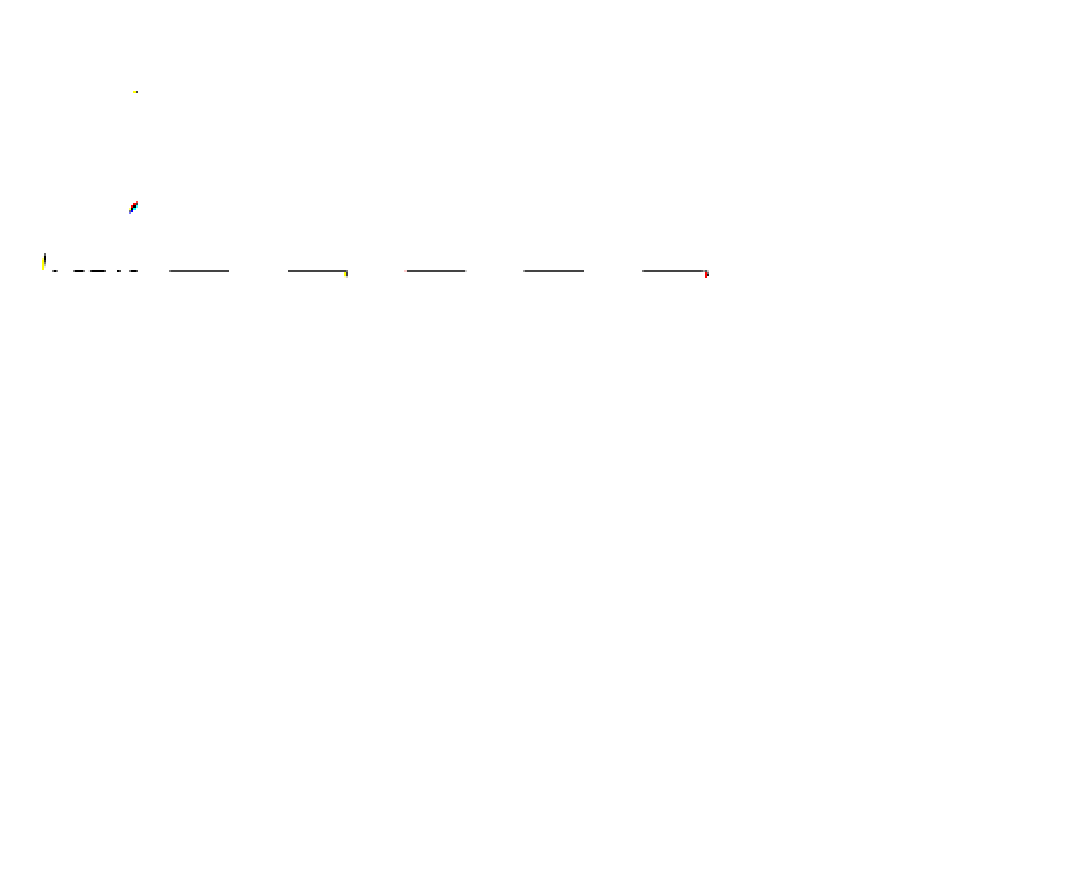
\includegraphics[width=0.5\columnwidth]{figures/triangular.pdf}
\caption{Triangular distribution $T(a, b, c)$}
\label{fig:triangular}
\end{figure}

\paragraph{Random Unreal (Figure 
~\ref{fig:Random-Unreal-Sample-Training-set})} The training set is 
sampled in a random uniform way, regardless of the file generation 
times. This method does not respect the time constraints in 
Equation~\ref{eq:time}, it will be used as a baseline for comparison 
with other methods.

In each method, we also included the first row of the matrix (first 
generated file of each subject) and a random column (all files of a 
random subject) to avoid cold start issues. 


\section{Datasets}

\label{sec:datasets}

\todo{Soudabeh, can you remove the caption on all matrices?}

\subsection{Synthetic Data}

We generated synthetic matrices as shown in 
Figure~\ref{fig:synthetic-data}. Each matrix has 100 files and 100 
subjects of different \emph{types}. Subjects of the same type behave 
identically and all types contain the same number of subjects $\pm$ 1. 
Such a decomposition by subject type correspond to the case where 
different subjects may have data of different nature, as it is for 
instance the case in the neuroimaging 
dataset of the Human Connectome Project~\cite{van2013wu} where not all the 
subjects have the same amount of images.

 For subjects of a given type, the reproducibility matrix consists of 
 $log(n)$  blocks, where $n$ is the number of types. Blocks are 
 arranged with all the possible variation patterns: some types do not 
 vary at all, while other ones vary in every block. Such variation 
 patterns are meant to mimic the logic of data 
processing pipelines: each block of files represents the files produced 
at a given stage of the pipeline, which may or may not contain 
reproducibility errors depending on the subject type.

\begin{figure}
\centering
        %\begin{subfigure}[b]{\columnwidth}
                  %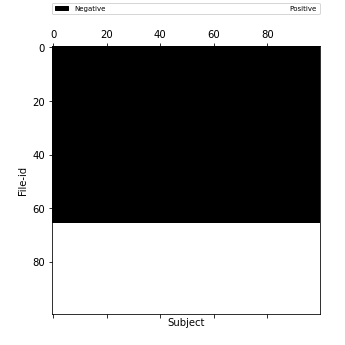
\includegraphics[width=\columnwidth]{data/Utility_Matrix/Synthetic/synthetic_subject_types/1_SubjectType_utility_matrix.png}
                  %\caption{1 type}
        %\end{subfigure}
        \begin{subfigure}[b]{0.45\columnwidth}
                  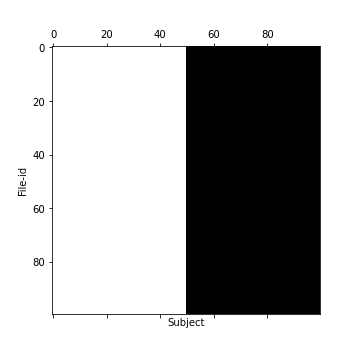
\includegraphics[width=\columnwidth]{data/Utility_Matrix/Synthetic/synthetic_subject_types/2_SubjectType_utility_matrix.png}
                  \caption{2 types}
        \end{subfigure}
        \begin{subfigure}[b]{0.45\columnwidth}
                  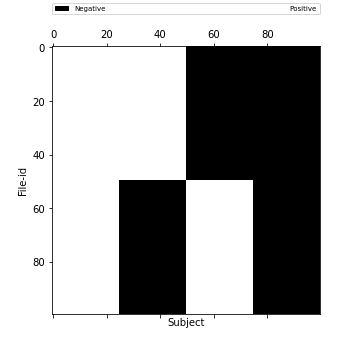
\includegraphics[width=\columnwidth]{data/Utility_Matrix/Synthetic/synthetic_subject_types/4_SubjectType_utility_matrix.png}
                  \caption{4 types}
        \end{subfigure}
                \begin{subfigure}[b]{0.45\columnwidth}
                  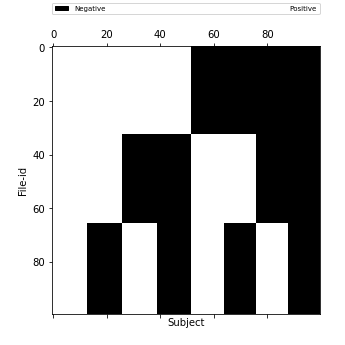
\includegraphics[width=\columnwidth]{data/Utility_Matrix/Synthetic/synthetic_subject_types/8_SubjectType_utility_matrix.png}
                  \caption{8 types}
        \end{subfigure}
                \begin{subfigure}[b]{0.45\columnwidth}
                  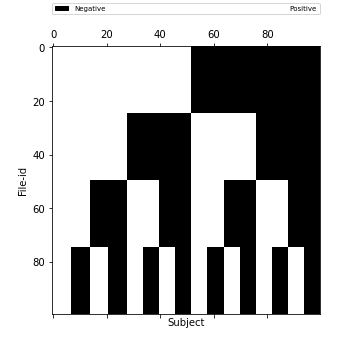
\includegraphics[width=\columnwidth]{data/Utility_Matrix/Synthetic/synthetic_subject_types/16_SubjectType_utility_matrix.png}
                  \caption{16 types}
        \end{subfigure}
                \begin{subfigure}[b]{0.45\columnwidth}
                  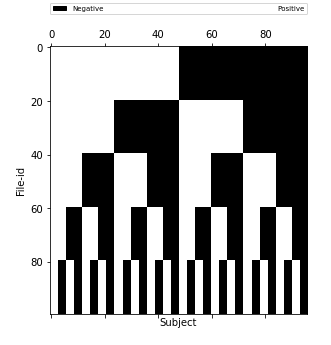
\includegraphics[width=\columnwidth]{data/Utility_Matrix/Synthetic/synthetic_subject_types/32_SubjectType_utility_matrix.png}
                  \caption{32 types}
        \end{subfigure}
                \begin{subfigure}[b]{0.45\columnwidth}
                  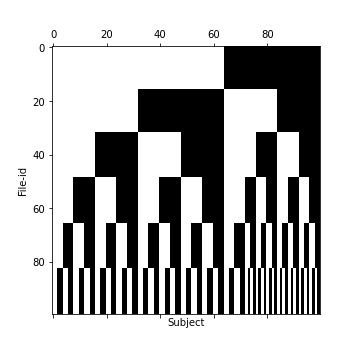
\includegraphics[width=\columnwidth]{data/Utility_Matrix/Synthetic/synthetic_subject_types/64_SubjectType_utility_matrix.png}
                  \caption{64 types}
        \end{subfigure}
\caption{Synthetic reproducibility matrices. White cells denote reproducibility errors.}
\label{fig:synthetic-data}
\end{figure}

\subsection{Real Data}

We collected data to evaluate the computational reproducibility of analysis
pipelines of the Human Connectome Project~\cite{glasser2013minimal}. We
processed a set S of 94 subjects randomly selected in the S500 HCP
release\footnote{\url{https://db.humanconnectome.org}} in three execution conditions with different
versions of the CentOS operating system (5.11, 6.8 and 7.2), using the
PreFreesurfer and Freesurfer pipelines described 
in~\cite{glasser2013minimal} and available on 
GitHub\footnote{\url{https://github.com/Washington-University/Pipelines/releases/tag/v3.19.0}}. 
For each pipeline, we identified the set F of files produced for all
subjects in all conditions. For each condition pair and each pipeline, 
we computed a binary reproducibility matrix U of size $|F|\times|S|$, 
where $U_{i,j}$ is true iif file $i$ of subject $j$ was different in 
each condition. Rows of $U$ were ordered by ascending file modification 
time in a random subject in S.

Figure~\ref{fig:utility-matrices} shows the utility matrices
obtained for the PreFreesurfer and Freesufer pipeline. The computational
reproducibility of these pipelines varies across subjects,
but some files behave
consistently across all subjects, leading to complete black or white
lines.
%The ratio of positive elements in utility matrix of CentOS5 vs CentOS6(C5C6),  CentOS5 vs CentOS7(C5C7) and  CentOS6 vs CentOS7(C6C7) are
%$0.34$, $0.79$ and $0.79$ respectively.

\begin{figure}[h!]
  \centering
  \begin{subfigure}[b]{0.45\columnwidth}
        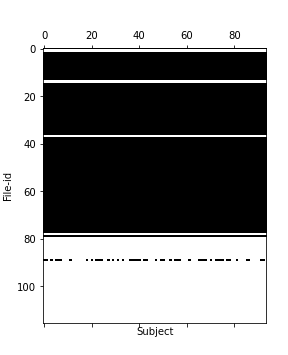
\includegraphics[width=\columnwidth]{data/Utility_Matrix/PreFreeSurfer/PFS_5v6_utility_matrix.png}
  \caption{PFS, C5 vs C6}
  \end{subfigure}
  \begin{subfigure}[b]{0.45\columnwidth}
         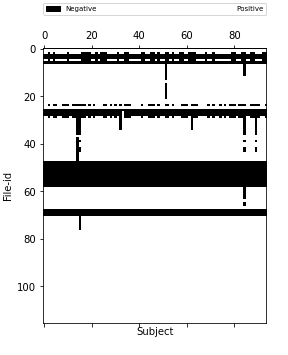
\includegraphics[width=\columnwidth]{data/Utility_Matrix/PreFreeSurfer/PFS_5v7_utility_matrix.png}
  \caption{PFS, C5 vs C7}
  \end{subfigure}
  \begin{subfigure}[b]{0.45\columnwidth}
        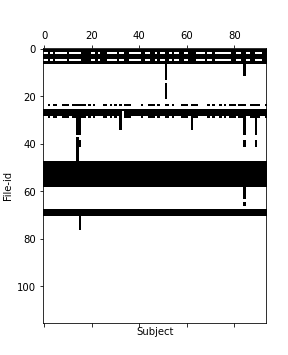
\includegraphics[width=\columnwidth]{data/Utility_Matrix/PreFreeSurfer/PFS_6v7_utility_matrix.png}
  \caption{PFS, C6 vs C7}
  \end{subfigure}
  \begin{subfigure}[b]{0.45\columnwidth}
        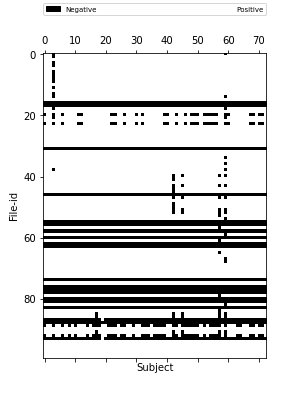
\includegraphics[width=\columnwidth]{data/Utility_Matrix/FS-100files/FS-First-bound-100files.png}
  \caption{FS (100 files), C6 vs C7}
  \end{subfigure}
  \caption{Utility matrices, PreFreesurfer (PFS) and Freesurfer (FS) pipelines}
    \label{fig:utility-matrices}
\end{figure}

\section{Results}

\label{sec:results}

Two experiments have been conducted for each reproducibility matrix, to evaluate the performance of our 
predictions using (1) ALS without biases, and (2) ALS with biases. 
Results will be evaluated using classification accuracy and compared to (1) a dummy classifier that always 
predicts the value in the majority class and (2) the Random Unreal 
method, used as the baseline sampling technique. All reported values are averages
over 5 repetitions. Due to sampling issues, it is possible that the actual 
training ratio obtained with some of the sampling methods does not 
match the target one. We checked that the difference between the target 
and real training ratios was lower than 0.01. We used Spark's ALS model 
as available in package \texttt{pyspark.ml}, with 50 factors, a 
regularization parameter of 0.01, a maximum of 5 iterations and non 
negative constraints set to true. \todo{Tristan: Add one plot with sensitivity and specificity for 0.9 training}

%~ , sensitivity and specificity defined as follows:
%~ \[
        %~ Accuracy = \frac{TP+TN}{TP+TN+FP+FN}
%~ \]
%~ \[
        %~ Sensitivity = \frac{TP}{TP+FN}
%~ \]
%~ \[
        %~ Specificity = \frac{TN}{TN+FP}
%~ \]
%~ Where TP is the number of True Positives (correctly predicted reproducibility errors), 
%~ FP is the number of False Positives, TN is the number of true negatives 
%~ and FN is the number of false negatives. \todo{Check if we want to report sensitivity and specificity, otherwise remove.}

\subsection{Synthetic Data}

\subsubsection{ALS without Bias}

Accuracy results for the different numbers of subject types are 
reported in Figure~\ref{fig:results-synthetic}. By construction, the 
accuracy of the dummy classifier is close to 0.5 for all subject types \todo{Soudabeh: why such variations?}. Random 
Unreal performs very well for all subject types, which confirms that 
ALS is working correctly. Unsurprisingly, all the other methods perform 
better than the dummy classifier, and their accuracy decreases as the 
number of subject types increases.

However, only 3 methods are able to provide accuracy values above 0.85 
for all subject types: Random Subjects (RS), RFNU and RFNTL. This is 
due to the fact that these methods are the only ones that can sample 
files produced toward the end of the execution while maintaining a 
reduced number of empty columns. Surprisingly, RFNTS does not perform 
well for more than 2 subject types, even for a training ratio of 0.9. \todo{Check that.}

RS, RFNU and RFNTL achieve a 90\% accuracy for a training ratio of 
about 0.85 \todo{precise that}. Therefore, 15\% of the computations could potentially be 
saved in such reproducibility studies.

\begin{figure*}
\begin{subfigure}[b]{\columnwidth}
        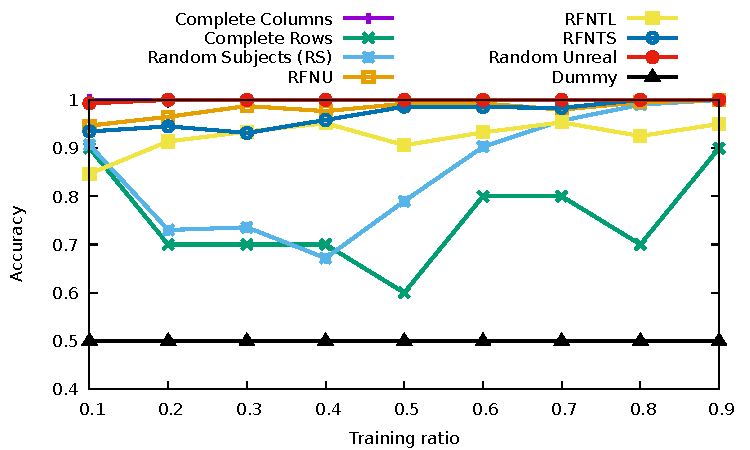
\includegraphics[width=0.8\columnwidth]{data/results/means_of_results/ALS/Synthetic/synthetic_subject_types/ALS-2-types.pdf}
        \caption{2 subject types}
\end{subfigure}
\begin{subfigure}[b]{\columnwidth}
        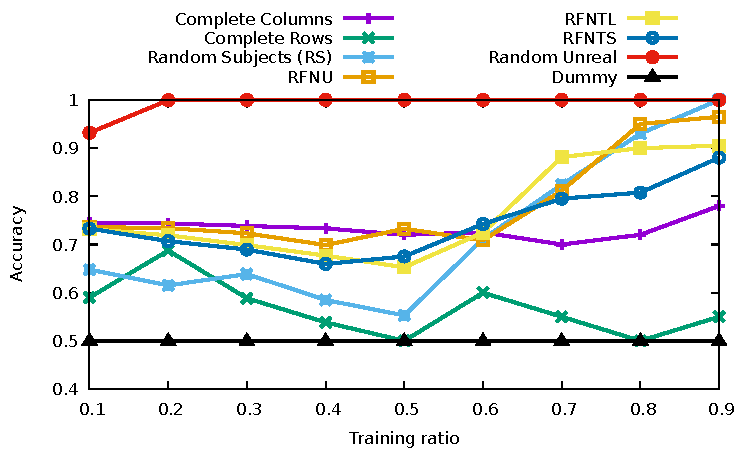
\includegraphics[width=0.8\columnwidth]{data/results/means_of_results/ALS/Synthetic/synthetic_subject_types/ALS-4-types.pdf}
        \caption{4 subject types}
\end{subfigure}
\begin{subfigure}[b]{\columnwidth}
        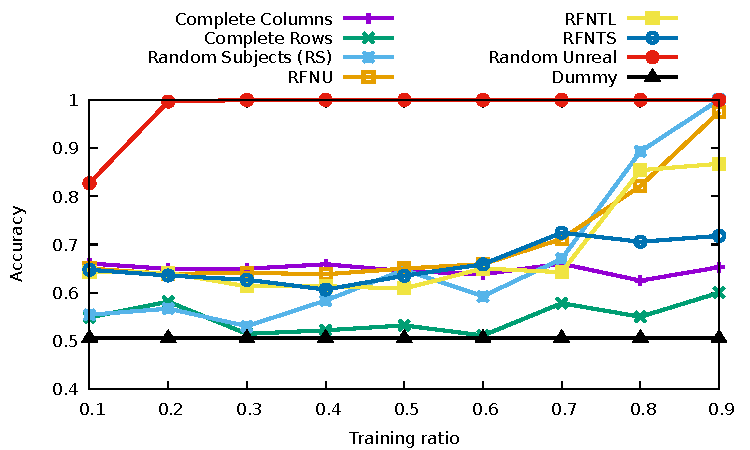
\includegraphics[width=0.8\columnwidth]{data/results/means_of_results/ALS/Synthetic/synthetic_subject_types/ALS-8-types.pdf}
        \caption{8 subject types}
\end{subfigure}
\begin{subfigure}[b]{\columnwidth}
        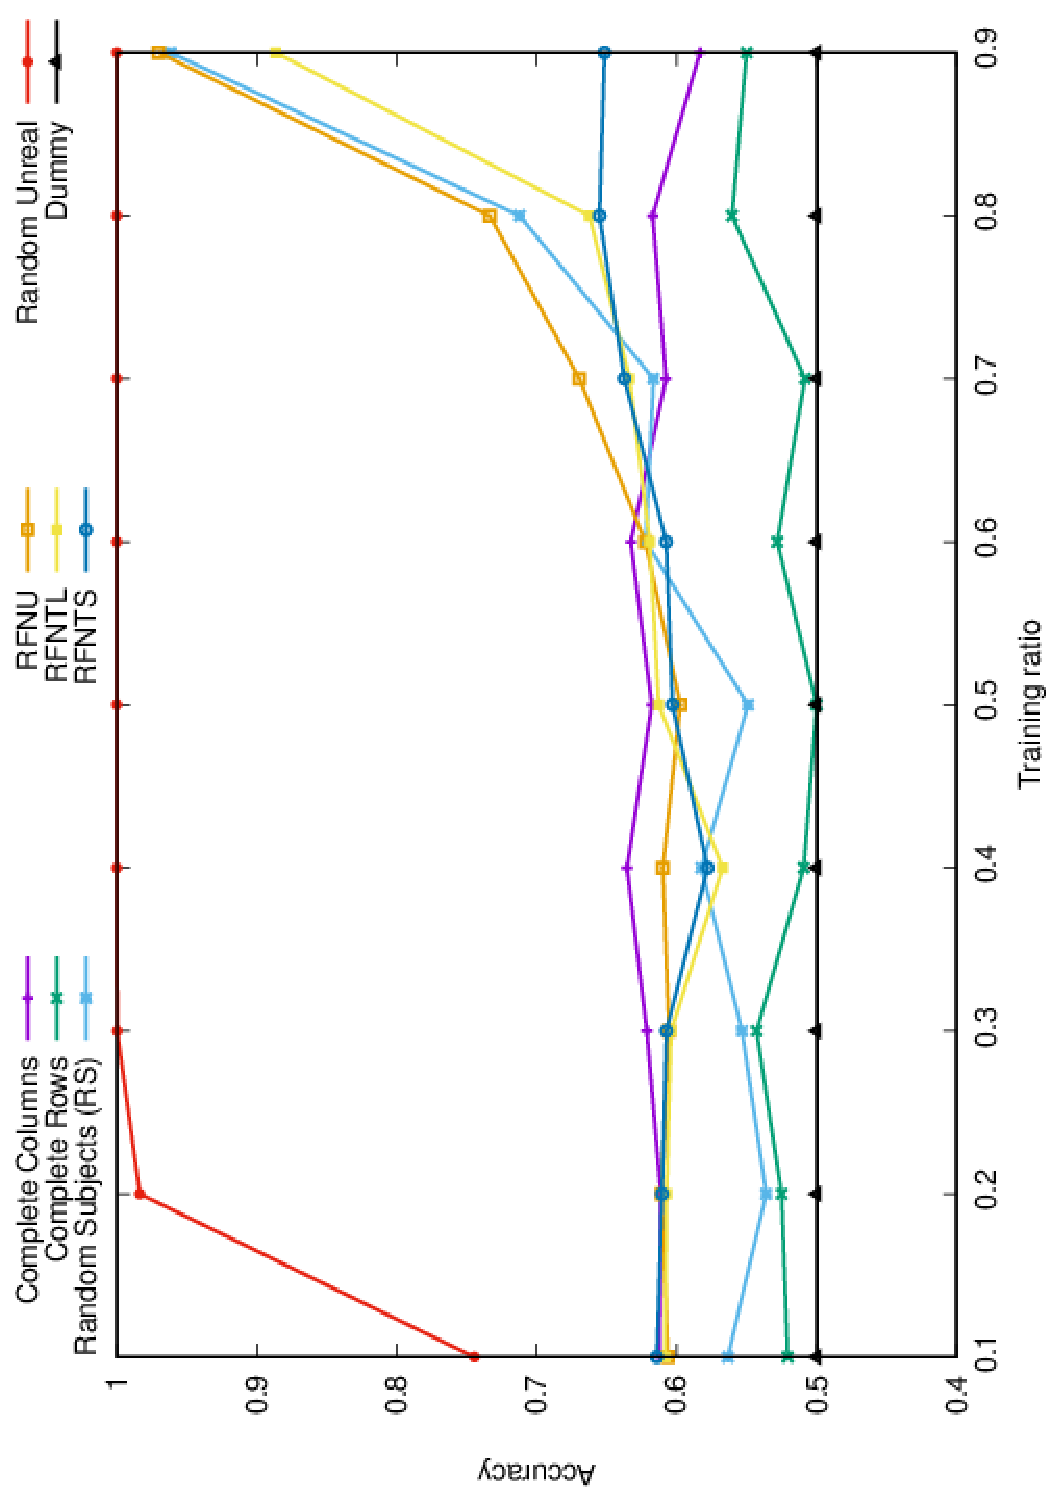
\includegraphics[width=0.8\columnwidth]{data/results/means_of_results/ALS/Synthetic/synthetic_subject_types/ALS-16-types.pdf}
        \caption{16 subject types}
\end{subfigure}
\begin{subfigure}[b]{\columnwidth}
        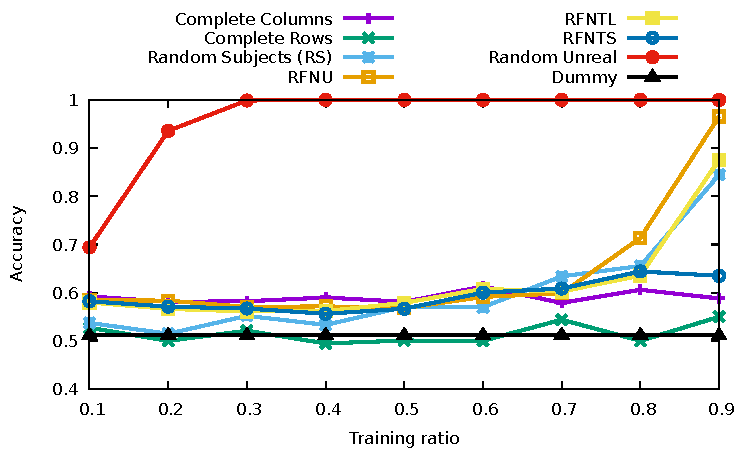
\includegraphics[width=0.8\columnwidth]{data/results/means_of_results/ALS/Synthetic/synthetic_subject_types/ALS-32-types.pdf}
        \caption{32 subject types}
\end{subfigure}
\hfill
\begin{subfigure}[b]{\columnwidth}
        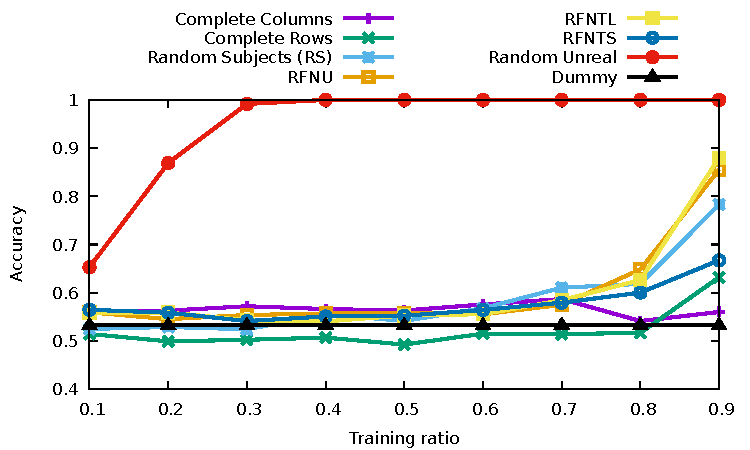
\includegraphics[width=0.8\columnwidth]{data/results/means_of_results/ALS/Synthetic/synthetic_subject_types/ALS-64-types.pdf}
        \caption{64 subject types}
\end{subfigure}
\caption{Accuracy results on synthetic data, ALS \emph{without} bias.}
\label{fig:results-synthetic}
\end{figure*}

\subsubsection{ALS with Bias}

Results of ALS with bias are reported in 
Figure~\ref{fig:results-synthetic-als-bias}. RS, RFNU and RFNTL remain 
the methods that best compare to Random Unreal, but the achieved 
accuracy is much lower than without Biases. This is presumably due to 
the fact that file biases are all close to 0.5 in the synthetic data. 
In such a situation, biases are detrimental to the accuracy of the 
collaborative filtering process and shouldn't be included.

\begin{figure*}
\begin{subfigure}[b]{\columnwidth}
        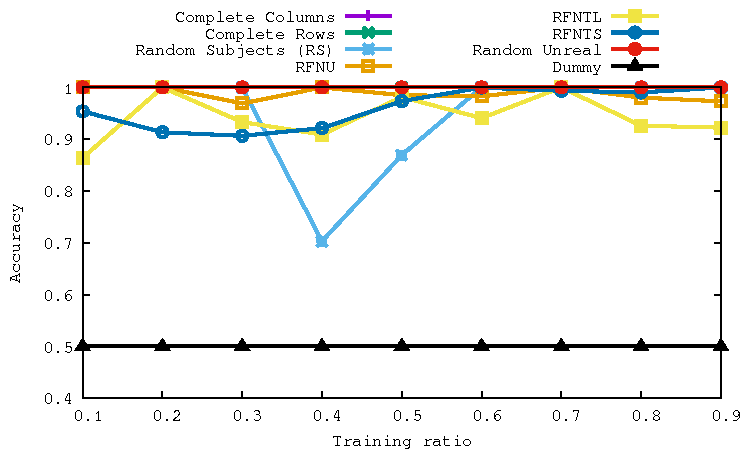
\includegraphics[width=0.8\columnwidth]{data/results/means_of_results/ALS-Bias/Synthetic/synthetic_subject_types/ALS-Bias-2-types.pdf}
        \caption{2 subject types}
\end{subfigure}
\begin{subfigure}[b]{\columnwidth}
        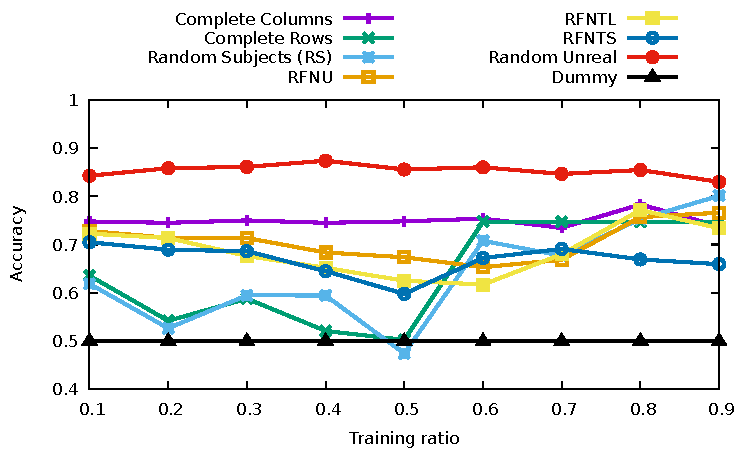
\includegraphics[width=0.8\columnwidth]{data/results/means_of_results/ALS-Bias/Synthetic/synthetic_subject_types/ALS-Bias-4-types.pdf}
        \caption{4 subject types}
\end{subfigure}
\begin{subfigure}[b]{\columnwidth}
        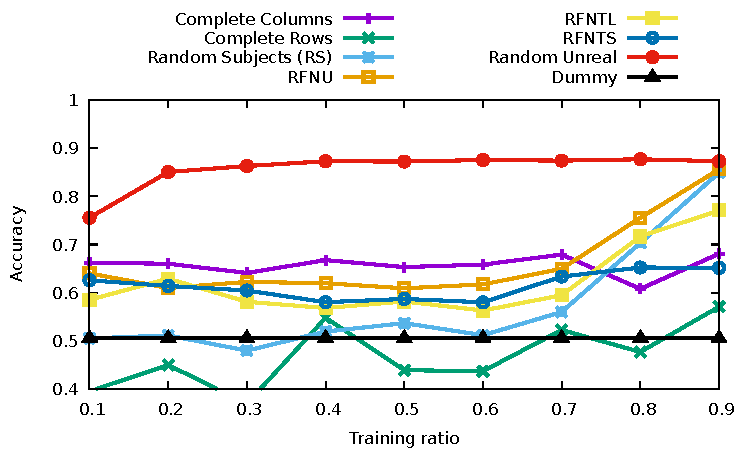
\includegraphics[width=0.8\columnwidth]{data/results/means_of_results/ALS-Bias/Synthetic/synthetic_subject_types/ALS-Bias-8-types.pdf}
        \caption{8 subject types}
\end{subfigure}
\begin{subfigure}[b]{\columnwidth}
        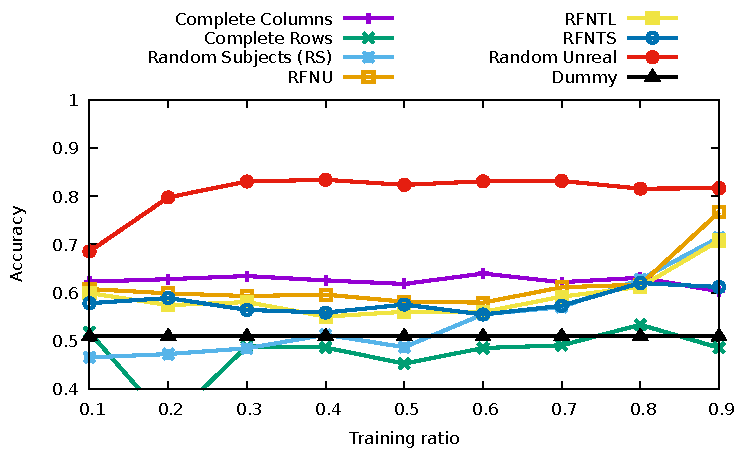
\includegraphics[width=0.8\columnwidth]{data/results/means_of_results/ALS-Bias/Synthetic/synthetic_subject_types/ALS-Bias-16-types.pdf}
        \caption{16 subject types}
\end{subfigure}
\begin{subfigure}[b]{\columnwidth}
        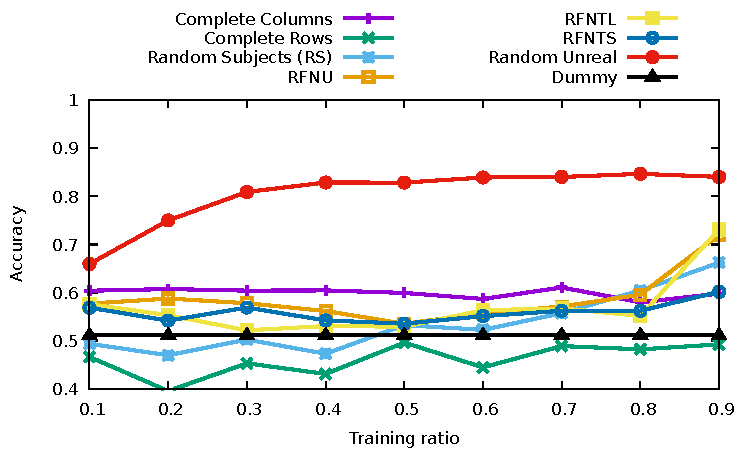
\includegraphics[width=0.8\columnwidth]{data/results/means_of_results/ALS-Bias/Synthetic/synthetic_subject_types/ALS-Bias-32-types.pdf}
        \caption{32 subject types}
\end{subfigure}
\hfill
\begin{subfigure}[b]{\columnwidth}
        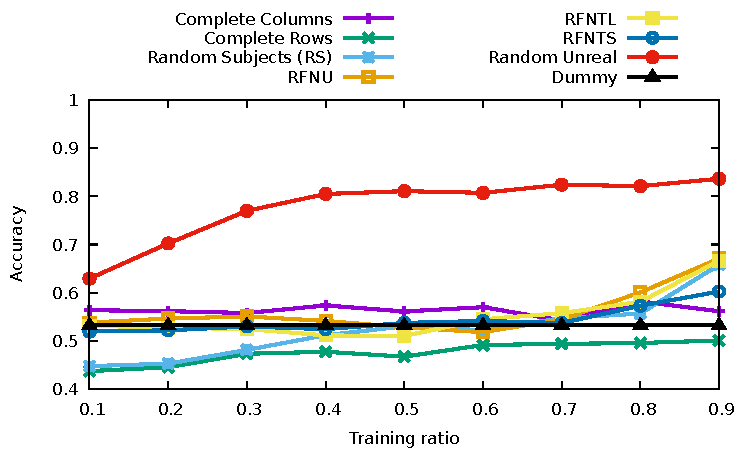
\includegraphics[width=0.8\columnwidth]{data/results/means_of_results/ALS-Bias/Synthetic/synthetic_subject_types/ALS-Bias-64-types.pdf}
        \caption{64 subject types}
\end{subfigure}
\caption{Accuracy results on synthetic data, ALS \emph{with} bias.}
\label{fig:results-synthetic-als-bias}
\end{figure*}

\subsection{Real Data}

\subsubsection{ALS without bias}

Results for ALS without bias are reported in 
Figure~\ref{fig:results-real-als}. Among the methods that performed 
well in the synthetic dataset, RFNU performs the best, with an accuracy 
higher than 0.95 for all datasets, when the training ratio is larger 
than 0.5. RS and RFNTL are slightly underperforming compared to RFNU. 
Complete rows and complete columns do not even reach the accuracy of 
the dummy classifier. The reference method, Random Unreal, has an 
accuracy close to 1, which shows that collaborative filtering works 
well on this dataset too.
\todo{why is the performance of columns so variable?}

\begin{figure*}
\begin{subfigure}[b]{\columnwidth}
        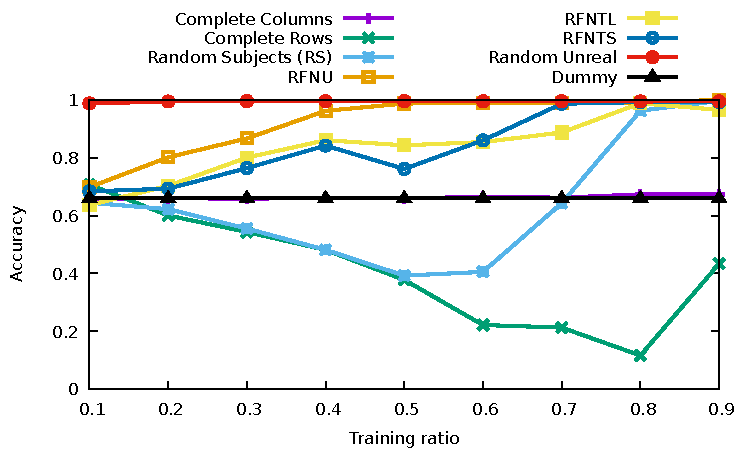
\includegraphics[width=0.8\columnwidth]{data/results/means_of_results/ALS/PreFreeSurfer/ALS-PFS-5v6.pdf}
        \caption{PFS, CentOS5 vs CentOS6}
\end{subfigure}
\begin{subfigure}[b]{\columnwidth}
        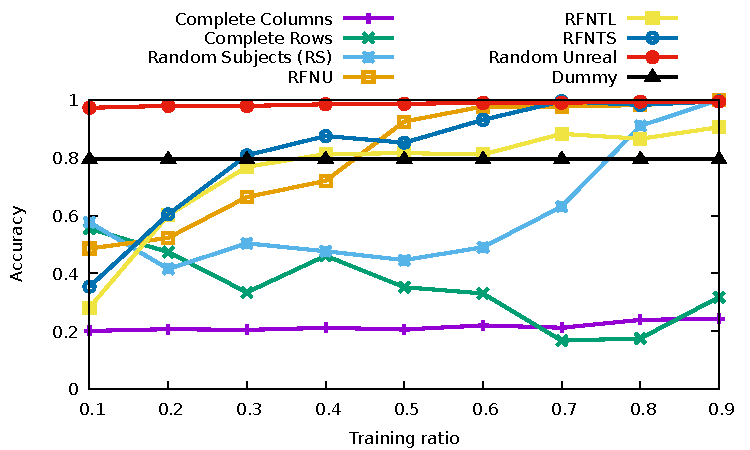
\includegraphics[width=0.8\columnwidth]{data/results/means_of_results/ALS/PreFreeSurfer/ALS-PFS-5v7.pdf}
        \caption{PFS, CentOS5 vs CentOS7}
\end{subfigure}
\begin{subfigure}[b]{\columnwidth}
        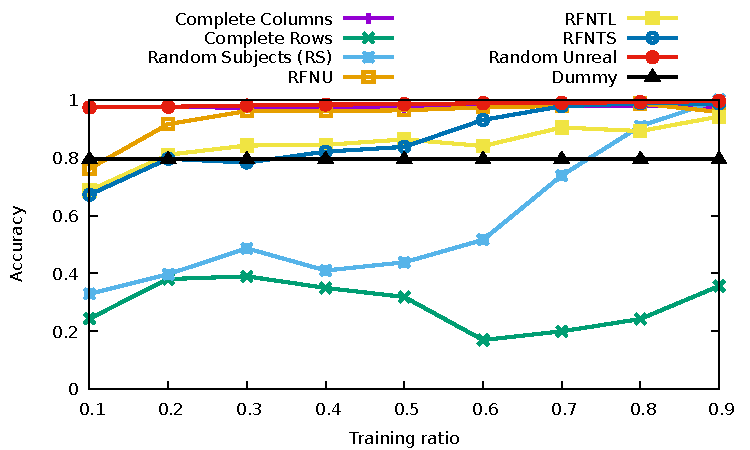
\includegraphics[width=0.8\columnwidth]{data/results/means_of_results/ALS/PreFreeSurfer/ALS-PFS-6v7.pdf}
        \caption{PFS, CentOS6 vs CentOS7}
\end{subfigure}\hfill
\begin{subfigure}[b]{\columnwidth}
        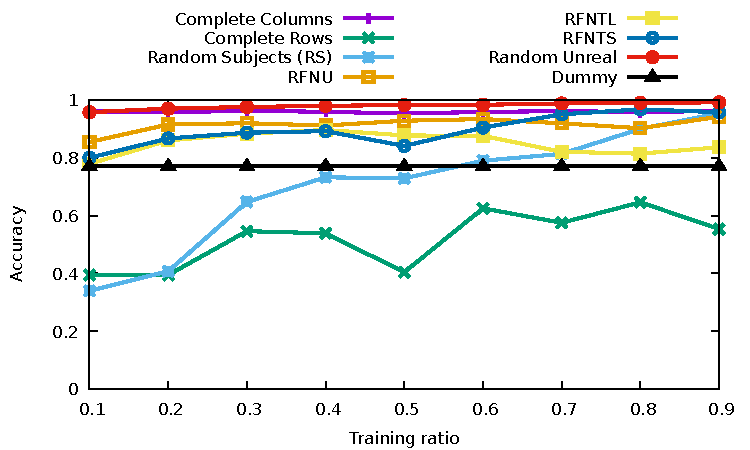
\includegraphics[width=0.8\columnwidth]{data/results/means_of_results/ALS/FS-100files/ALS-FS100files.pdf}
        \caption{FS, CentOS6 vs CentOS7}
\end{subfigure}
\caption{Accuracy results on PreFresurfer (PFS) and Freesurfer (FS) data, ALS \emph{without} bias.}
\label{fig:results-real-als}
\end{figure*}

\subsubsection{ALS with bias}

Results for ALS with bias are reported in 
Figure~\ref{fig:results-real-als-bias}. From a training ratio of 0.5, 
all methods have a very good accuracy for all datasets, except complete 
columns in Figure~\ref{fig:pfs-c5vsc7-bias}. All methods except RFNU, 
RFNTL and RFNTS also perform well for a training ratio lower than 0.5. 
Overall, the accuracy of the methods is much higher than without bias. 
This is because the file bias is very strong in this dataset, as 
illustrated by the large number of constant lines in the matrices in 
Figure~\ref{fig:utility-matrices}.

\begin{figure*}
\begin{subfigure}[b]{\columnwidth}
        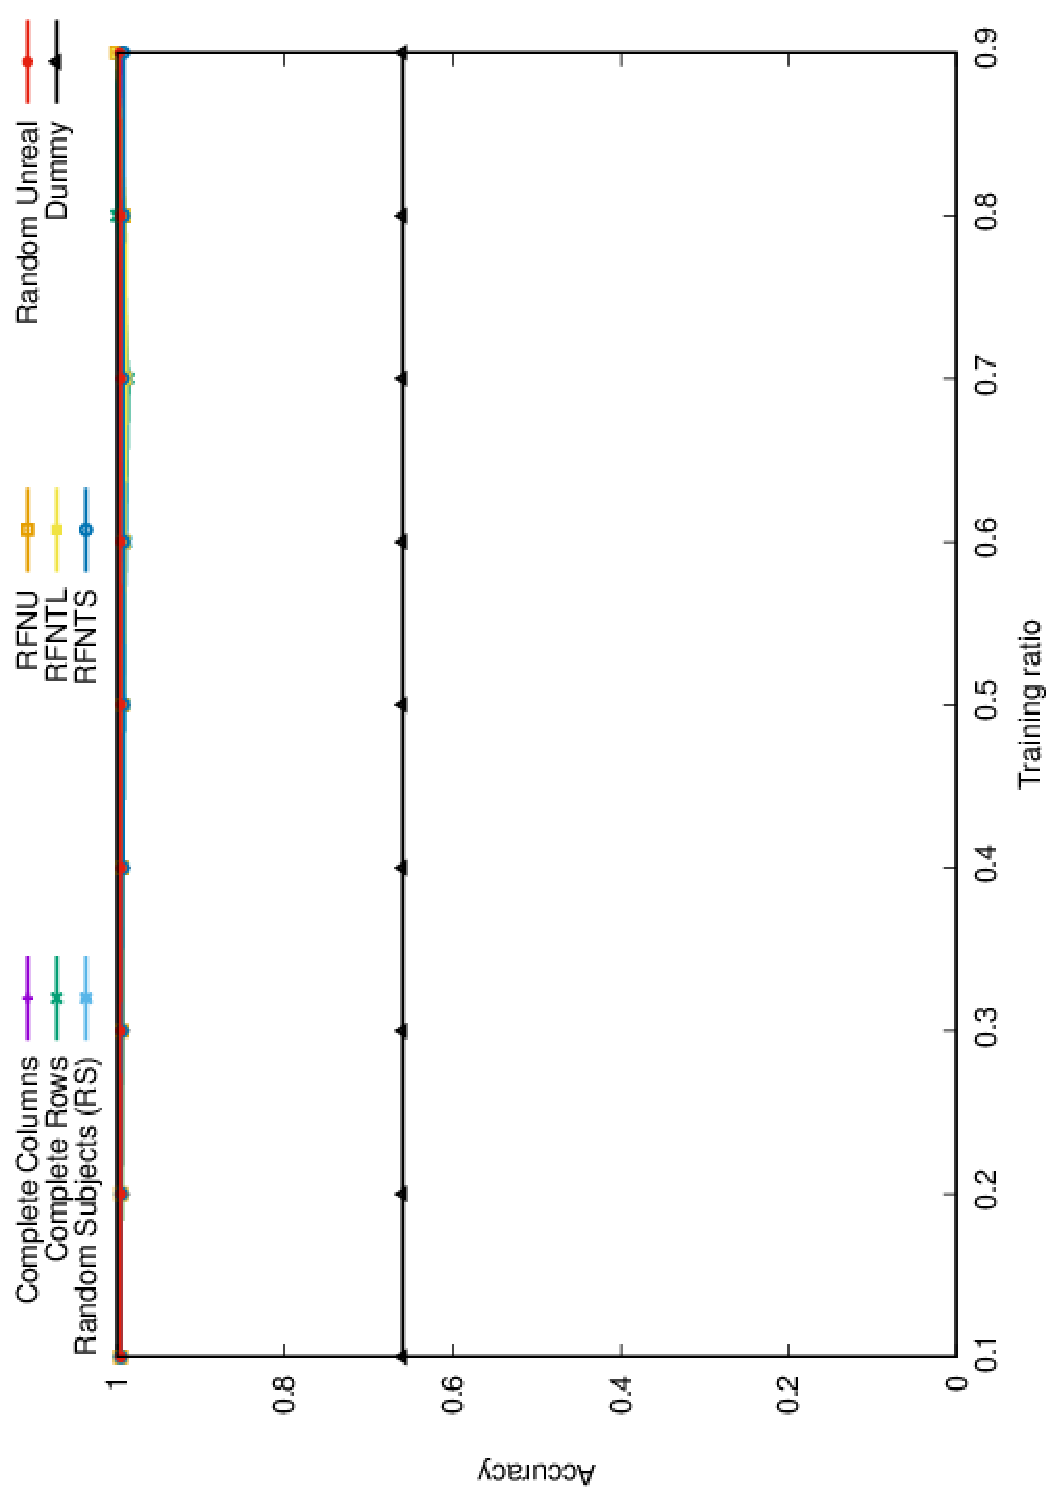
\includegraphics[width=0.8\columnwidth]{data/results/means_of_results/ALS-Bias/PreFreeSurfer/ALS-Bias-PFS-5v6.pdf}
        \caption{PFS, CentOS5 vs CentOS6}
\end{subfigure}
\begin{subfigure}[b]{\columnwidth}
        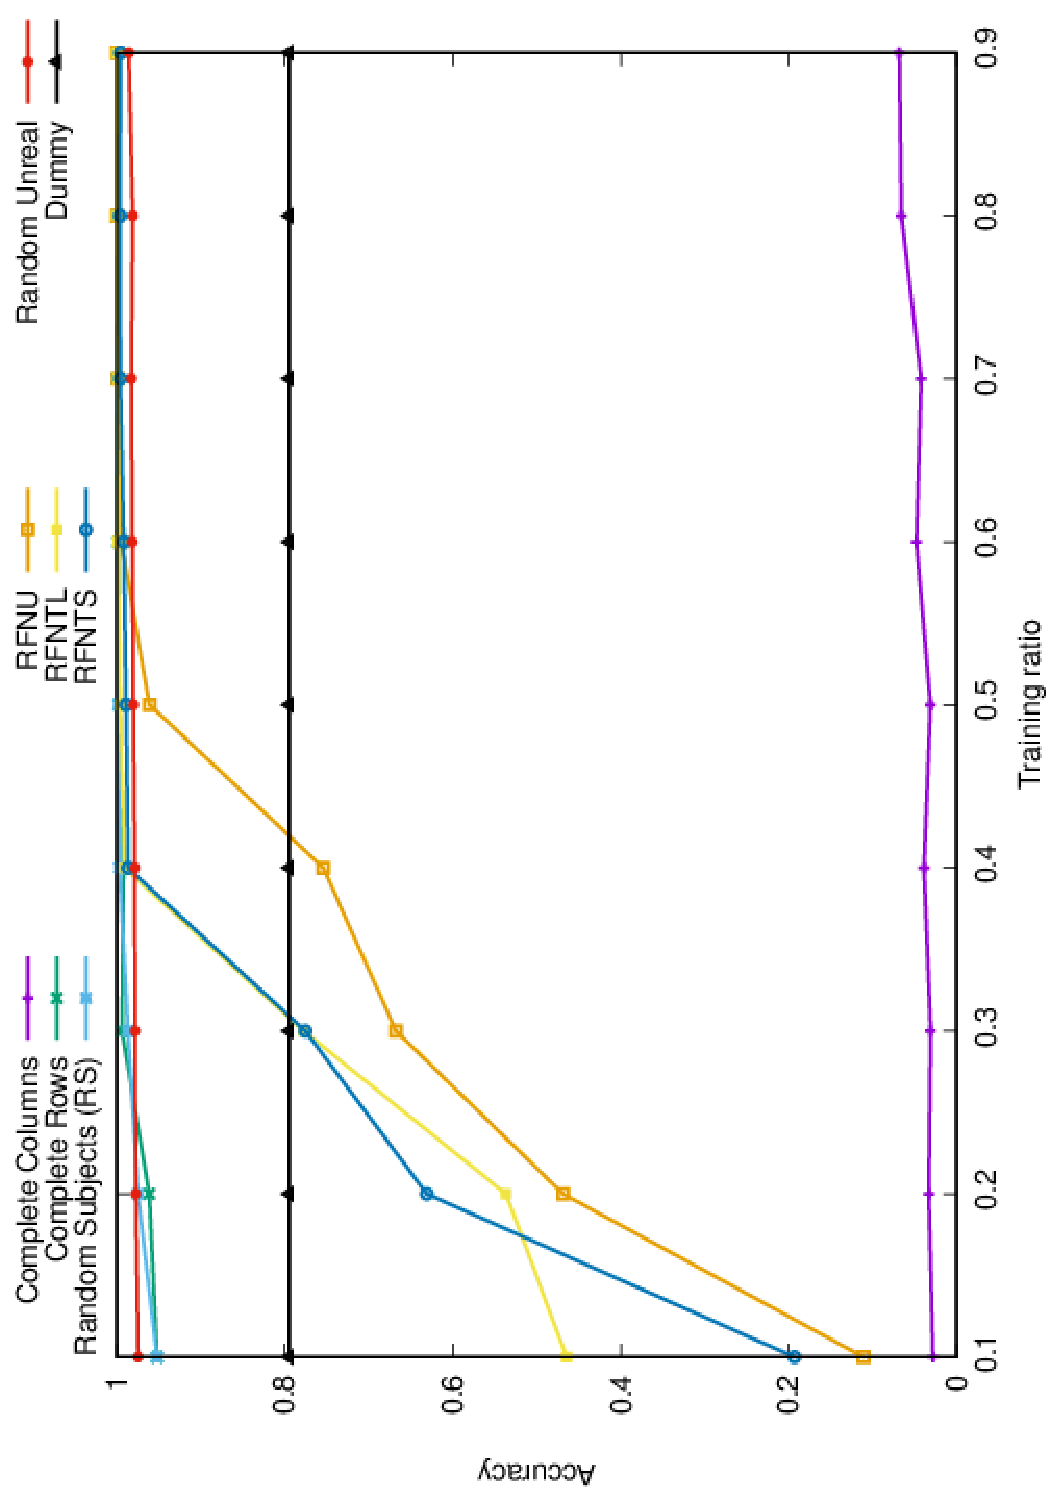
\includegraphics[width=0.8\columnwidth]{data/results/means_of_results/ALS-Bias/PreFreeSurfer/ALS-Bias-PFS-5v7.pdf}
        \caption{PFS, CentOS5 vs CentOS7}
        \label{fig:pfs-c5vsc7-bias}
\end{subfigure}
\begin{subfigure}[b]{\columnwidth}
        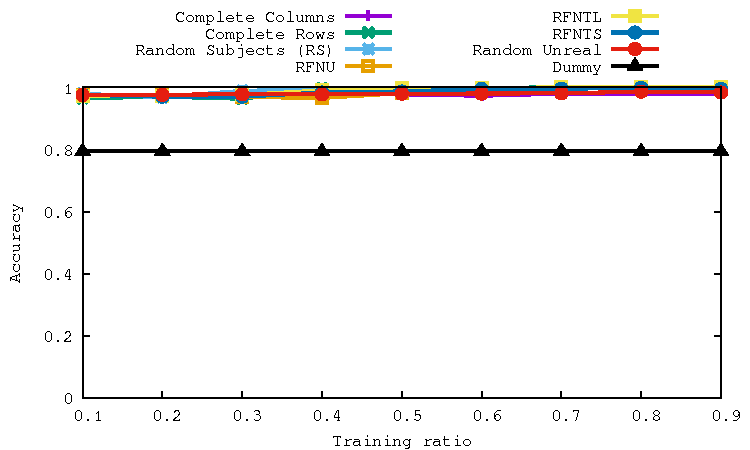
\includegraphics[width=0.8\columnwidth]{data/results/means_of_results/ALS-Bias/PreFreeSurfer/ALS-Bias-PFS-6v7.pdf}
        \caption{PFS, CentOS6 vs CentOS7}
\end{subfigure}\hfill
\begin{subfigure}[b]{\columnwidth}
        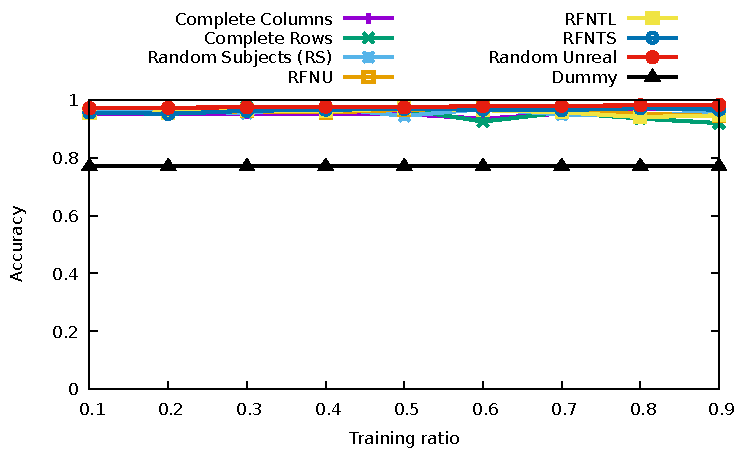
\includegraphics[width=0.8\columnwidth]{data/results/means_of_results/ALS-Bias/FS-100files/ALS-Bias-FS100files.pdf}
        \caption{FS, CentOS6 vs CentOS7}
\end{subfigure}
\caption{Accuracy results on PreFresurfer (PFS) and Freesurfer (FS) data, ALS \emph{with} bias.}
\label{fig:results-real-als-bias}
\end{figure*}

\subsubsection{ROC analysis}

Figure~\ref{fig:roc} compares the sampling methods in the ROC space, 
for a training ratio of 0.9, on the synthetic and Freesurfer dataset. 
The PreFreesurfer dataset is not included since specificity of RFNTL, 
RFNU, RS and complete rows is undefined at this training ratio (the 
test set only contains positive elements \todo{check matrix with 
Soudabeh to confirm}). The average sensitivity and specificity values 
are reported in Table~\ref{table:roc}. On average, RFNU is the best 
performing method.

\begin{figure*}
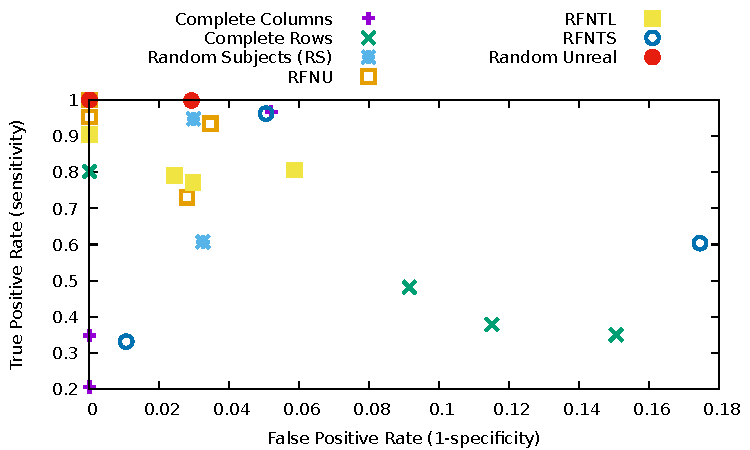
\includegraphics[width=\columnwidth]{data/results/roc/roc.pdf}
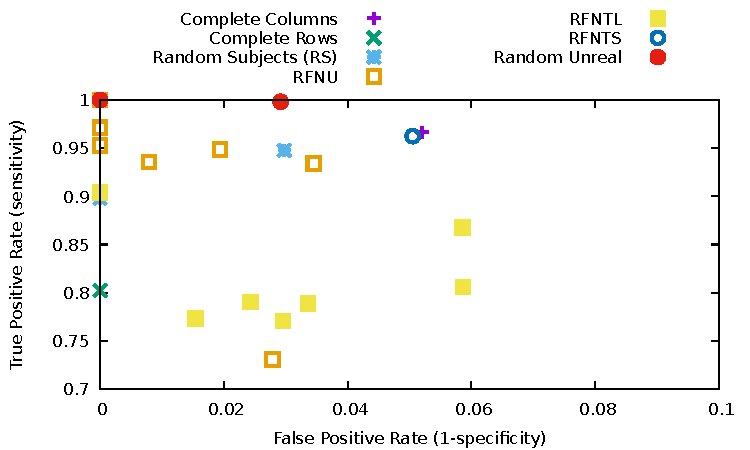
\includegraphics[width=\columnwidth]{data/results/roc/roc-closeup.pdf}
\caption{Comparison of the sampling methods in the ROC space for the 6 synthetic datasets and Freesurfer. Right: entire dataset. Left: close-up on the top-left part.}
\label{fig:roc}
\end{figure*}

\begin{table}
\centering
\begin{tabular}{ccc}
& Sensitivity & Specificity \\
\hline
Complete Columns & 0.53 & 0.97\\
Complete Rows & 0.43 & 0.89\\
Random Subjects & 0.88 & 0.99\\
RFNU & 0.92 & 0.99 \\
RFNTL & 0.81 & 0.97\\
RFNTS & 0.65 & 0.93 \\
Random Unreal & 1 & 1
\end{tabular}
\caption{Average sensitivity and specificity values for the 6 synthetic datasets and Freesurfer.}
\label{table:roc}
\end{table}

\subsection{Effect of the number of factors}
\todo{Soudabeh: Different number of factors: type 8, RFNU, 50, 100, 200, 400.}

\section{Discussion}

% Which method is the best
While collaborative filtering, perhaps unsurprisingly, is able to 
correctly predict the missing values in a matrix modeling the 
reproducibility problem, the usual random sampling method cannot be 
used in time-constrained processes. We proposed 6 sampling methods to 
address this issue, and we found that one of them, RFNU, \todo{check 
that} is consistently able to solve the problem. We explain that by 
the fact that RFNU leads the training set to contain a balanced mix 
between nearly complete and nearly empty columns, with a continuum of 
intermediate configurations in between. On the contrary, other sampling 
methods, including RFNTL and RFNTS, bias the sampling toward complete 
or empty columns, which is sometimes detrimental to accuracy.

Figure~\ref{fig:overlap} illustrates the comparison between RFNU, RFNTL 
and RFNTS. The matrices in this Figure represent the union between the 
training and the test set, where the training set is represented in 
black (negatives) and white (positives), and the test set is 
represented in green (true positives), yellow (false negatives), gray 
(true negatives) and red (false positives). This representation 
provides insights regarding where, and perhaps why, prediction errors 
occur. At this training ratio, RFNU (Figure~\ref{fig:overlap-rfntu}) 
uniformly samples the number of files per subject between 0.8$N_f$ and 
$N_f$. It provides an opportunity for ALS to be trained on the last 
files of the pipelines, while maintaining a low number of columns with 
a low training ratio. On the contrary, RFNTL 
(Figure~\ref{fig:overlap-rfntl}) samples the number of files per 
subject from 0.85$N_f$, but the probability to have a complete column 
is 0 (the one complete column in Figure~\ref{fig:overlap-rfntl} is the 
one included to prevent cold start issues), which leads to a "stripe" 
of errors at the bottom of the matrix. RFNTS 
(Figure~\ref{fig:overlap-rfnts}) doesn't have this issue, as it 
includes many complete columns in the training set, but this comes at 
the cost of several columns with a very low number of files, lower than 
60\%. For such columns, the prediction may go somewhat wrong, which explains
the reduced accuracy compared to RFNU.

\begin{figure*}
\begin{subfigure}[b]{0.6\columnwidth}
        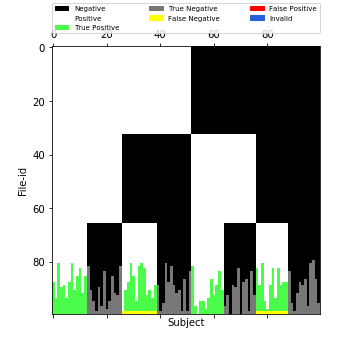
\includegraphics[width=\columnwidth]{figures/RFNU_Syn_8_ALS_09_test_data_matrix_run1.png}
        \caption{RFNU: $U(0.8N_f, N_f)$}
        \label{fig:overlap-rfnu}
\end{subfigure}
\hfill
\begin{subfigure}[b]{0.6\columnwidth}
        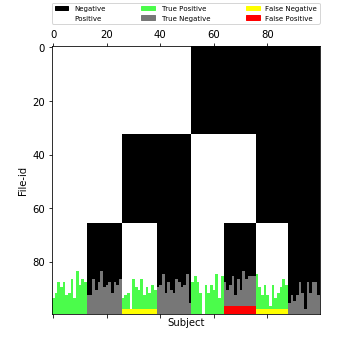
\includegraphics[width=\columnwidth]{figures/RFNT-L_Syn_8_ALS_09_test_data_matrix_run2.png}
        \caption{RFNTL: $T(0.85N_f, 0.85N_f, N_f)$}
        \label{fig:overlap-rfntl}
\end{subfigure}
\hfill
\begin{subfigure}[b]{0.6\columnwidth}
        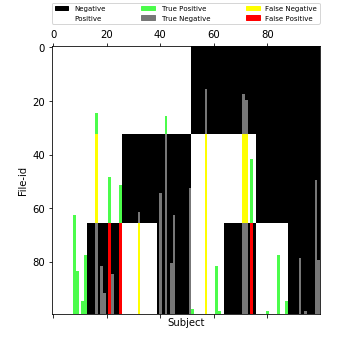
\includegraphics[width=\columnwidth]{figures/RFNT-S_Syn_8_ALS_09_test_data_matrix_run1.png}
        \caption{RFNTS: 0.3$T(0, N_f, N_f)$+0.7$N_f$}
        \label{fig:overlap-rfnts}
\end{subfigure}
\caption{Comparison between RFNU, RFNTL and RFNTS on synthetic dataset with 8 types, $\alpha=0.9$.}
\label{fig:overlap}
\end{figure*}

% Training ratio
On datasets that are strongly dependent on row bias, such as the real 
datasets studied here, RFNU provides accuracy values that are 
consistently higher than 0.95 for training ratios higher than 0.5, even 
when biases are not included in the collaborative filtering 
optimization. On the synthetic dataset, RFNU still performs very well 
when biases are not included. However, the training ratio required to 
reach a 0.95 accuracy increases with the number of subject types 
present in the dataset. \todo{maybe find a relation between the 
required training ratio and the number of subjects per subject type in 
the entire dataset}

In any case, we recommend not to include biases in the collaborative filtering 
optimization to solve this problem. Even though biases provide a slight 
accuracy improvement when datasets are strongly biased (constant lines 
in the matrix), they can also be very detrimental for more complex 
datasets such as the synthetic one used here.

% How can this be used in practice
From a practical standpoint, our study shows that reproducibility 
evaluations can be conducted using only 50\% of the files produced by 
the evaluated pipelines, with an accuracy above 95\%. Potentially, this 
could reduce the computing time and storage required for such studies 
by a factor of 2. However, such studies could not be conducted by 
processing only half of the subjects entirely, which would correspond 
to the Complete Columns sampling method. Instead, the processing of all 
the subjects should be initiated, and it should be terminated in a random
uniform way, assuming that files are uniformly produced throughout the 
execution.

% What are the limitations
Our study could be extended by considering real-valued reproducibility 
matrices instead of just binary ones. It is indeed common for file 
differences to be quantified using specific similarity measures or 
distances, such as Levenshtein distance between strings, or the sum of 
squared distances between voxels of an image. Our sampling methods 
could be directly applied to real-valued matrices, and we expect our 
conclusions regarding the best-performing sampling method (RFNU) and 
the inclusion of biases in the model to remain valid.

% Other possible examples
The method described in this paper and applied to reproducibility 
studies could be used to predict the other variables controlled by 
hidden, deterministic, hidden, parameterized, time-dependent processes, 
for instance markers of chronicle disease activity. In the 
reproducibility example studied in this paper, the variable of interest 
is the reproducibility of files produced by the processing of a given 
subjects, the process is the evaluated pipeline, it is hidden since we 
consider the pipeline as a black box (we don't inspect its source 
code), it is parametrized as it behaves differently on different input 
datasets and parameters, it is time-dependent as the value of the 
variable of interest varies throughout the course of the pipeline 
execution. 

\todo{Discussion on points that are not part of constant lines. Soudabeh: add an overlap matrix for FS, RFNU, ALS, at 0.5 or 0.6.}

\todo{Make sure the code is available and results are reproducible. Soudabeh: push your code to reprotools. Tristan: release and check.}

\section*{Acknowledgement}

We thank Compute Canada for providing the compute and storage resources
required for this study.

\bibliographystyle{IEEEtran}
\bibliography{IEEEabrv,biblio.bib}


\end{document}
